\documentclass[a4paper,12pt]{article}
\usepackage{amsmath,amssymb,amsfonts,amsthm}
\usepackage{tikz}
\usepackage [utf8x] {inputenc}
\usepackage [T2A] {fontenc} 
\usepackage[russian]{babel}
\usepackage{cmap} 
\usepackage{ gensymb }
% Так ссылки в PDF будут активны
\usepackage[unicode]{hyperref}
\usepackage{ textcomp }
\usepackage{indentfirst}
\usepackage[version=3]{mhchem}

% вы сможете вставлять картинки командой \includegraphics[width=0.7\textwidth]{ИМЯ ФАЙЛА}
% получается подключать, как минимум, файлы .pdf, .jpg, .png.
\usepackage{graphicx}
% Если вы хотите явно указать поля:
\usepackage[margin=1in]{geometry}
% Или если вы хотите задать поля менее явно (чем больше DIV, тем больше места под текст):
% \usepackage[DIV=10]{typearea}

\usepackage{fancyhdr}

\newcommand{\bbR}{\mathbb R}%теперь вместо длинной команды \mathbb R (множество вещественных чисел) можно писать короткую запись \bbR. Вместо \bbR вы можете вписать любую строчку букв, которая начинается с '\'.
\newcommand{\eps}{\varepsilon}
\newcommand{\bbN}{\mathbb N}
\newcommand{\dif}{\mathrm{d}}

\newtheorem{Def}{Определение}


\pagestyle{fancy}
\makeatletter % сделать "@" "буквой", а не "спецсимволом" - можно использовать "служебные" команды, содержащие @ в названии
\fancyhead[L]{\footnotesize Лабораторные работы по общей физике}%Это будет написано вверху страницы слева
\fancyhead[R]{\footnotesize ФУПМ МФТИ}
%\fancyfoot[L]{\footnotesize \@author}%имя автора будет написано внизу страницы слева
\fancyfoot[R]{\thepage}%номер страницы —- внизу справа
\fancyfoot[C]{}%по центру внизу страницы пусто

\renewcommand{\maketitle}{%
	\noindent{\bfseries\scshape\large\@title\ \mdseries\upshape}\par
	\noindent {\large\itshape\@author}
	\vskip 2ex}
\makeatother
\def\dd#1#2{\frac{\partial#1}{\partial#2}}


\title{2.1. Опыт Франка-Герца}
\author{Хурсик Екатерина} 

\begin{document}	
\maketitle


\section{Цель работы}
    Измерить энергию первого уровня атома гелия в динамическом и статическом 
    режимах методом электронного возбуждения.
\section{Метод достижения цели}

    Чтобы измерить энергию первого уровня атома гелия в динамическом режиме
    методом элеткронного возбуждения, делаем следующее:
    \begin{itemize}
        \item получаем по экрану осциллографа вольт-амперную характеристику $I_k=f(V_a)$;
        \item При максимальном ускоряющем напряжении измеряем на экране расстояние между минимумами;
        \item Вычисляем по найденному расстоянию энергию.
    \end{itemize}
    Чтобы измерить энергию первого уровня атома гелия в статическом режиме
    методом элеткронного возбуждения, нужно:
    \begin{itemize}
        \item снять зависимость коллектороного тока от анодного напряжения $I_k=f(V_a)$ (особенно тщательно проводим измерения в тех областях, где наблюдаются минимумы и максимумы)
        \item по полученной зависимости строим поточечно график;
        \item по графику измеряем расстояние между минимумами;
        \item находим по этому расстоянию эниргию.
    \end{itemize}
\newpage
\section{Ход работы}
    Сначала получим вольт-амперную характеристику $I_K=f(V_a)$ в динамическом режиме.
    Для трех значений задерживающего напряжения получим осциллограммы.
    Цена деления осциллографа $5B$.
    
    \begin{figure}[h!]
        \begin{center}
            \begin{minipage}{0.32\textwidth}
                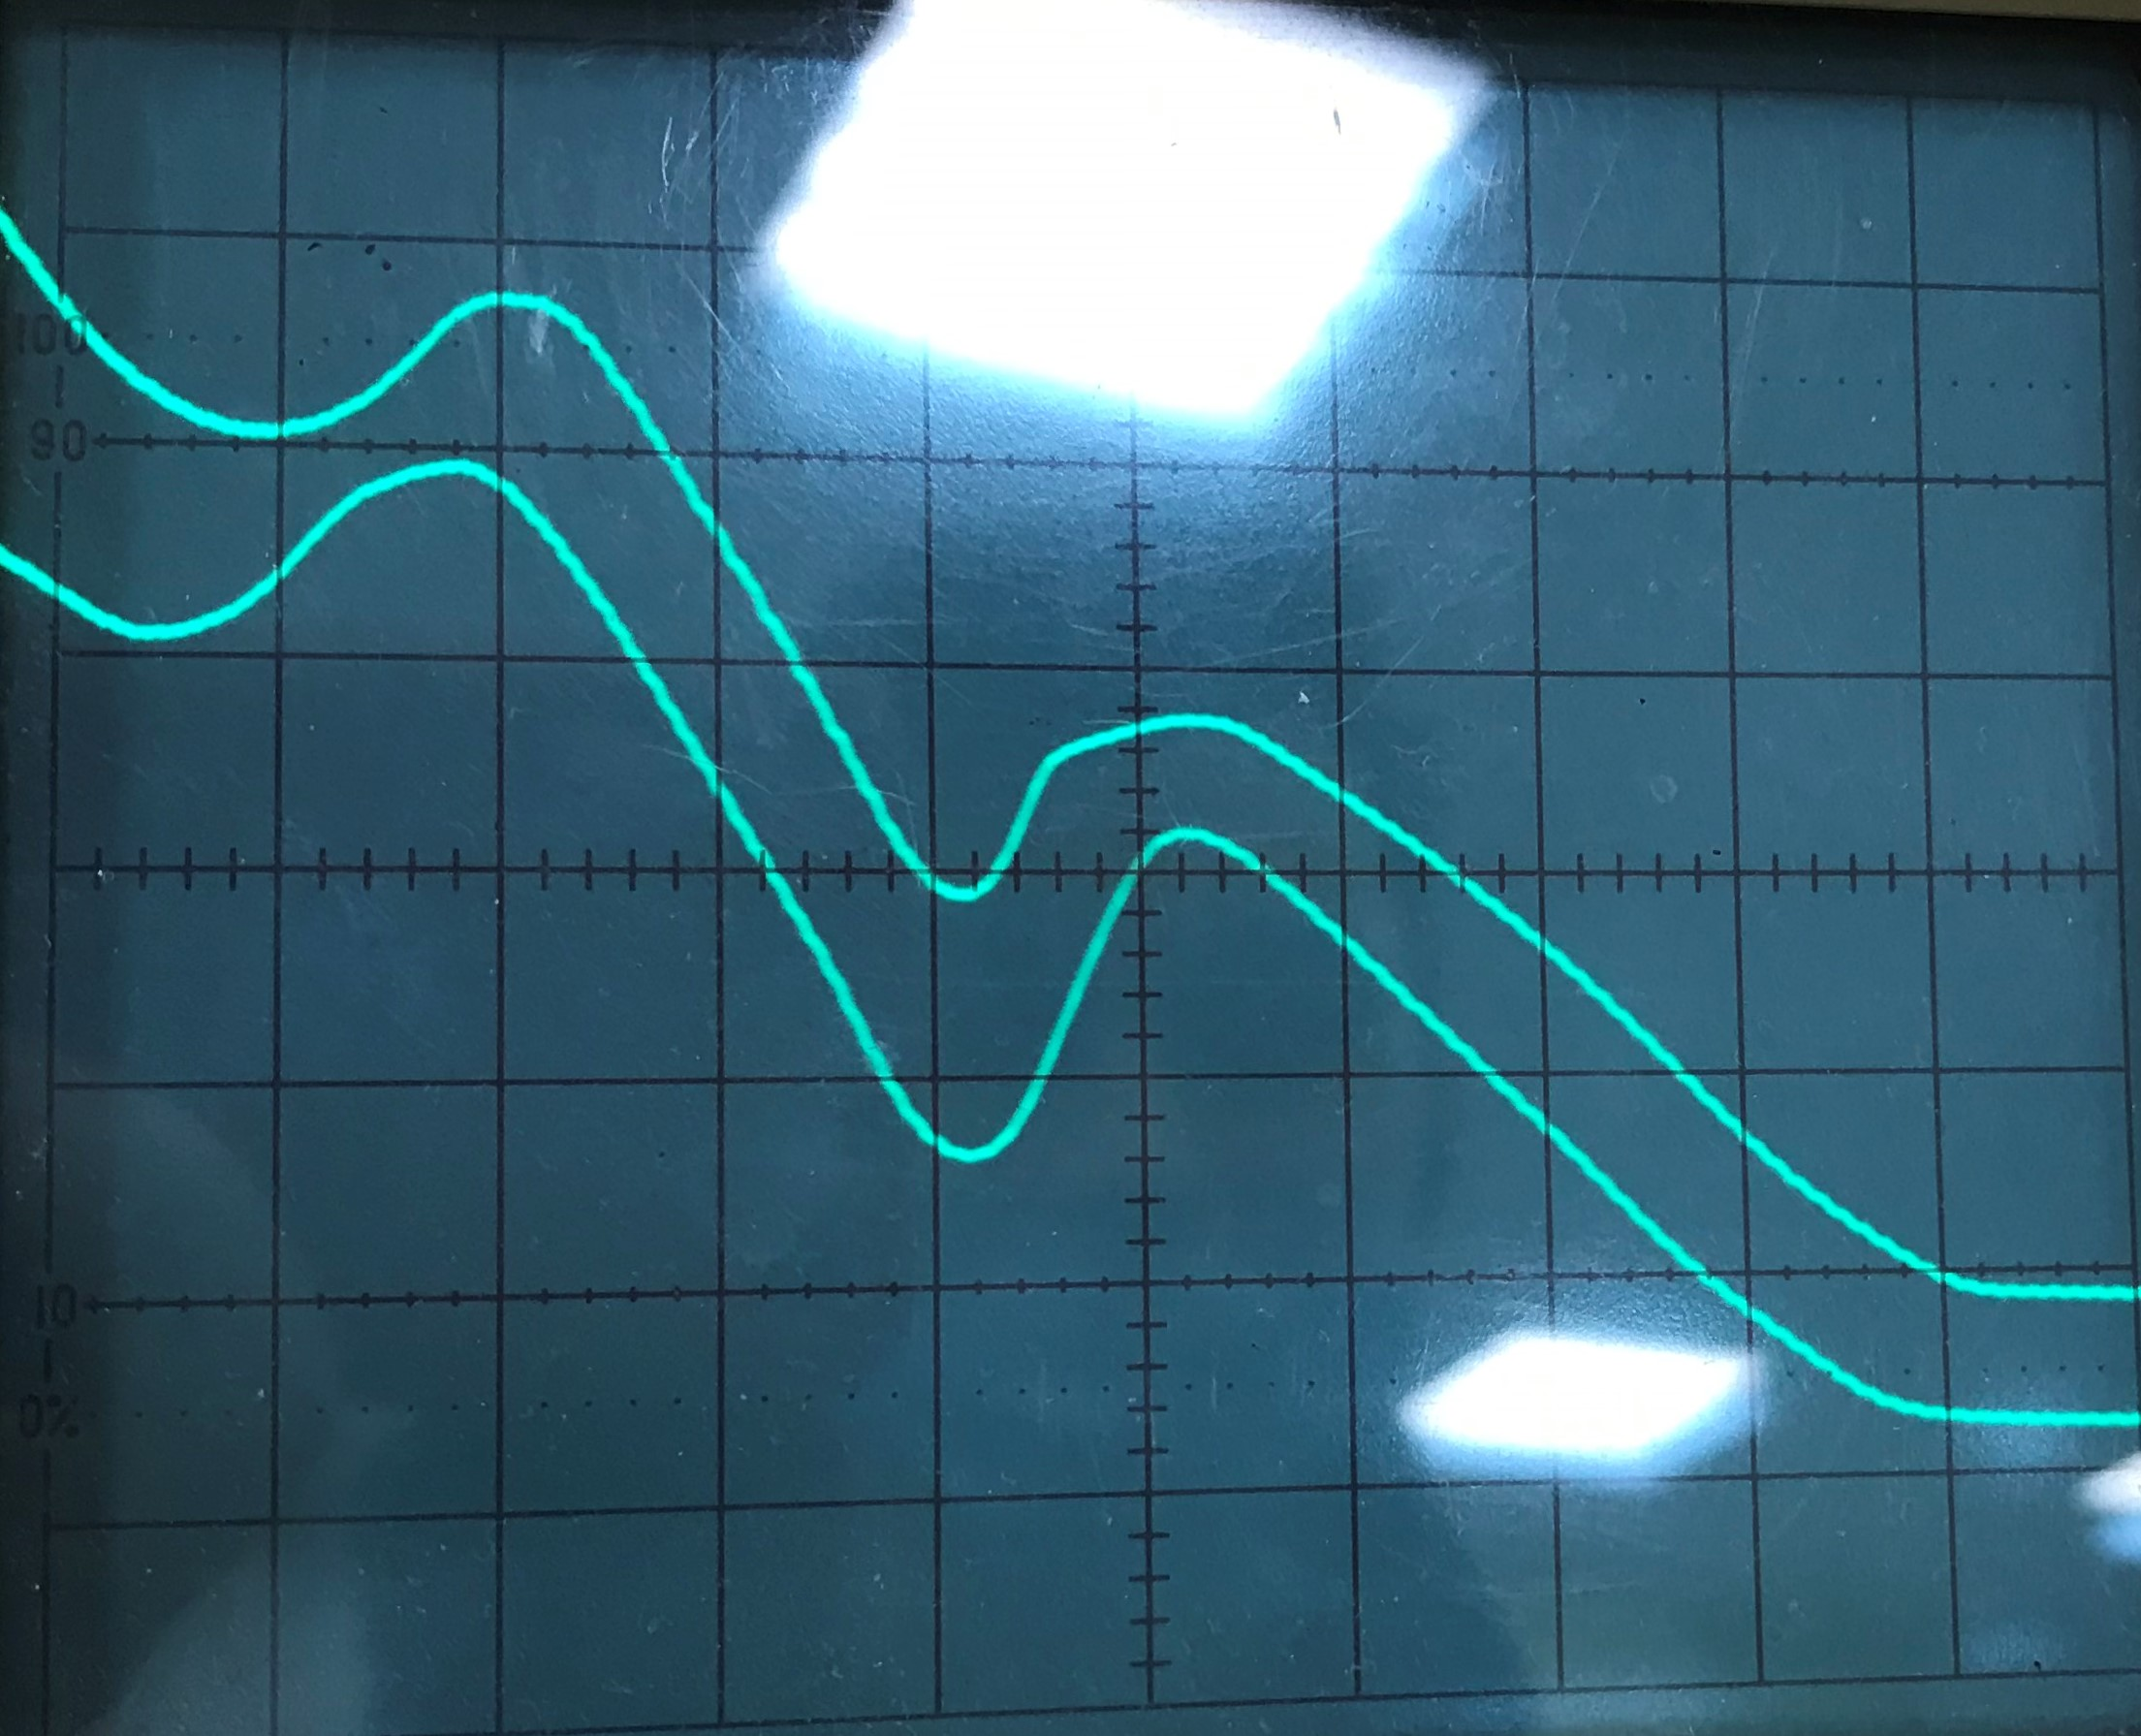
\includegraphics[width=\textwidth]{4}
                \caption{$U = 4V$}
            \end{minipage}
            \hfill
            \begin{minipage}{0.32\textwidth}
                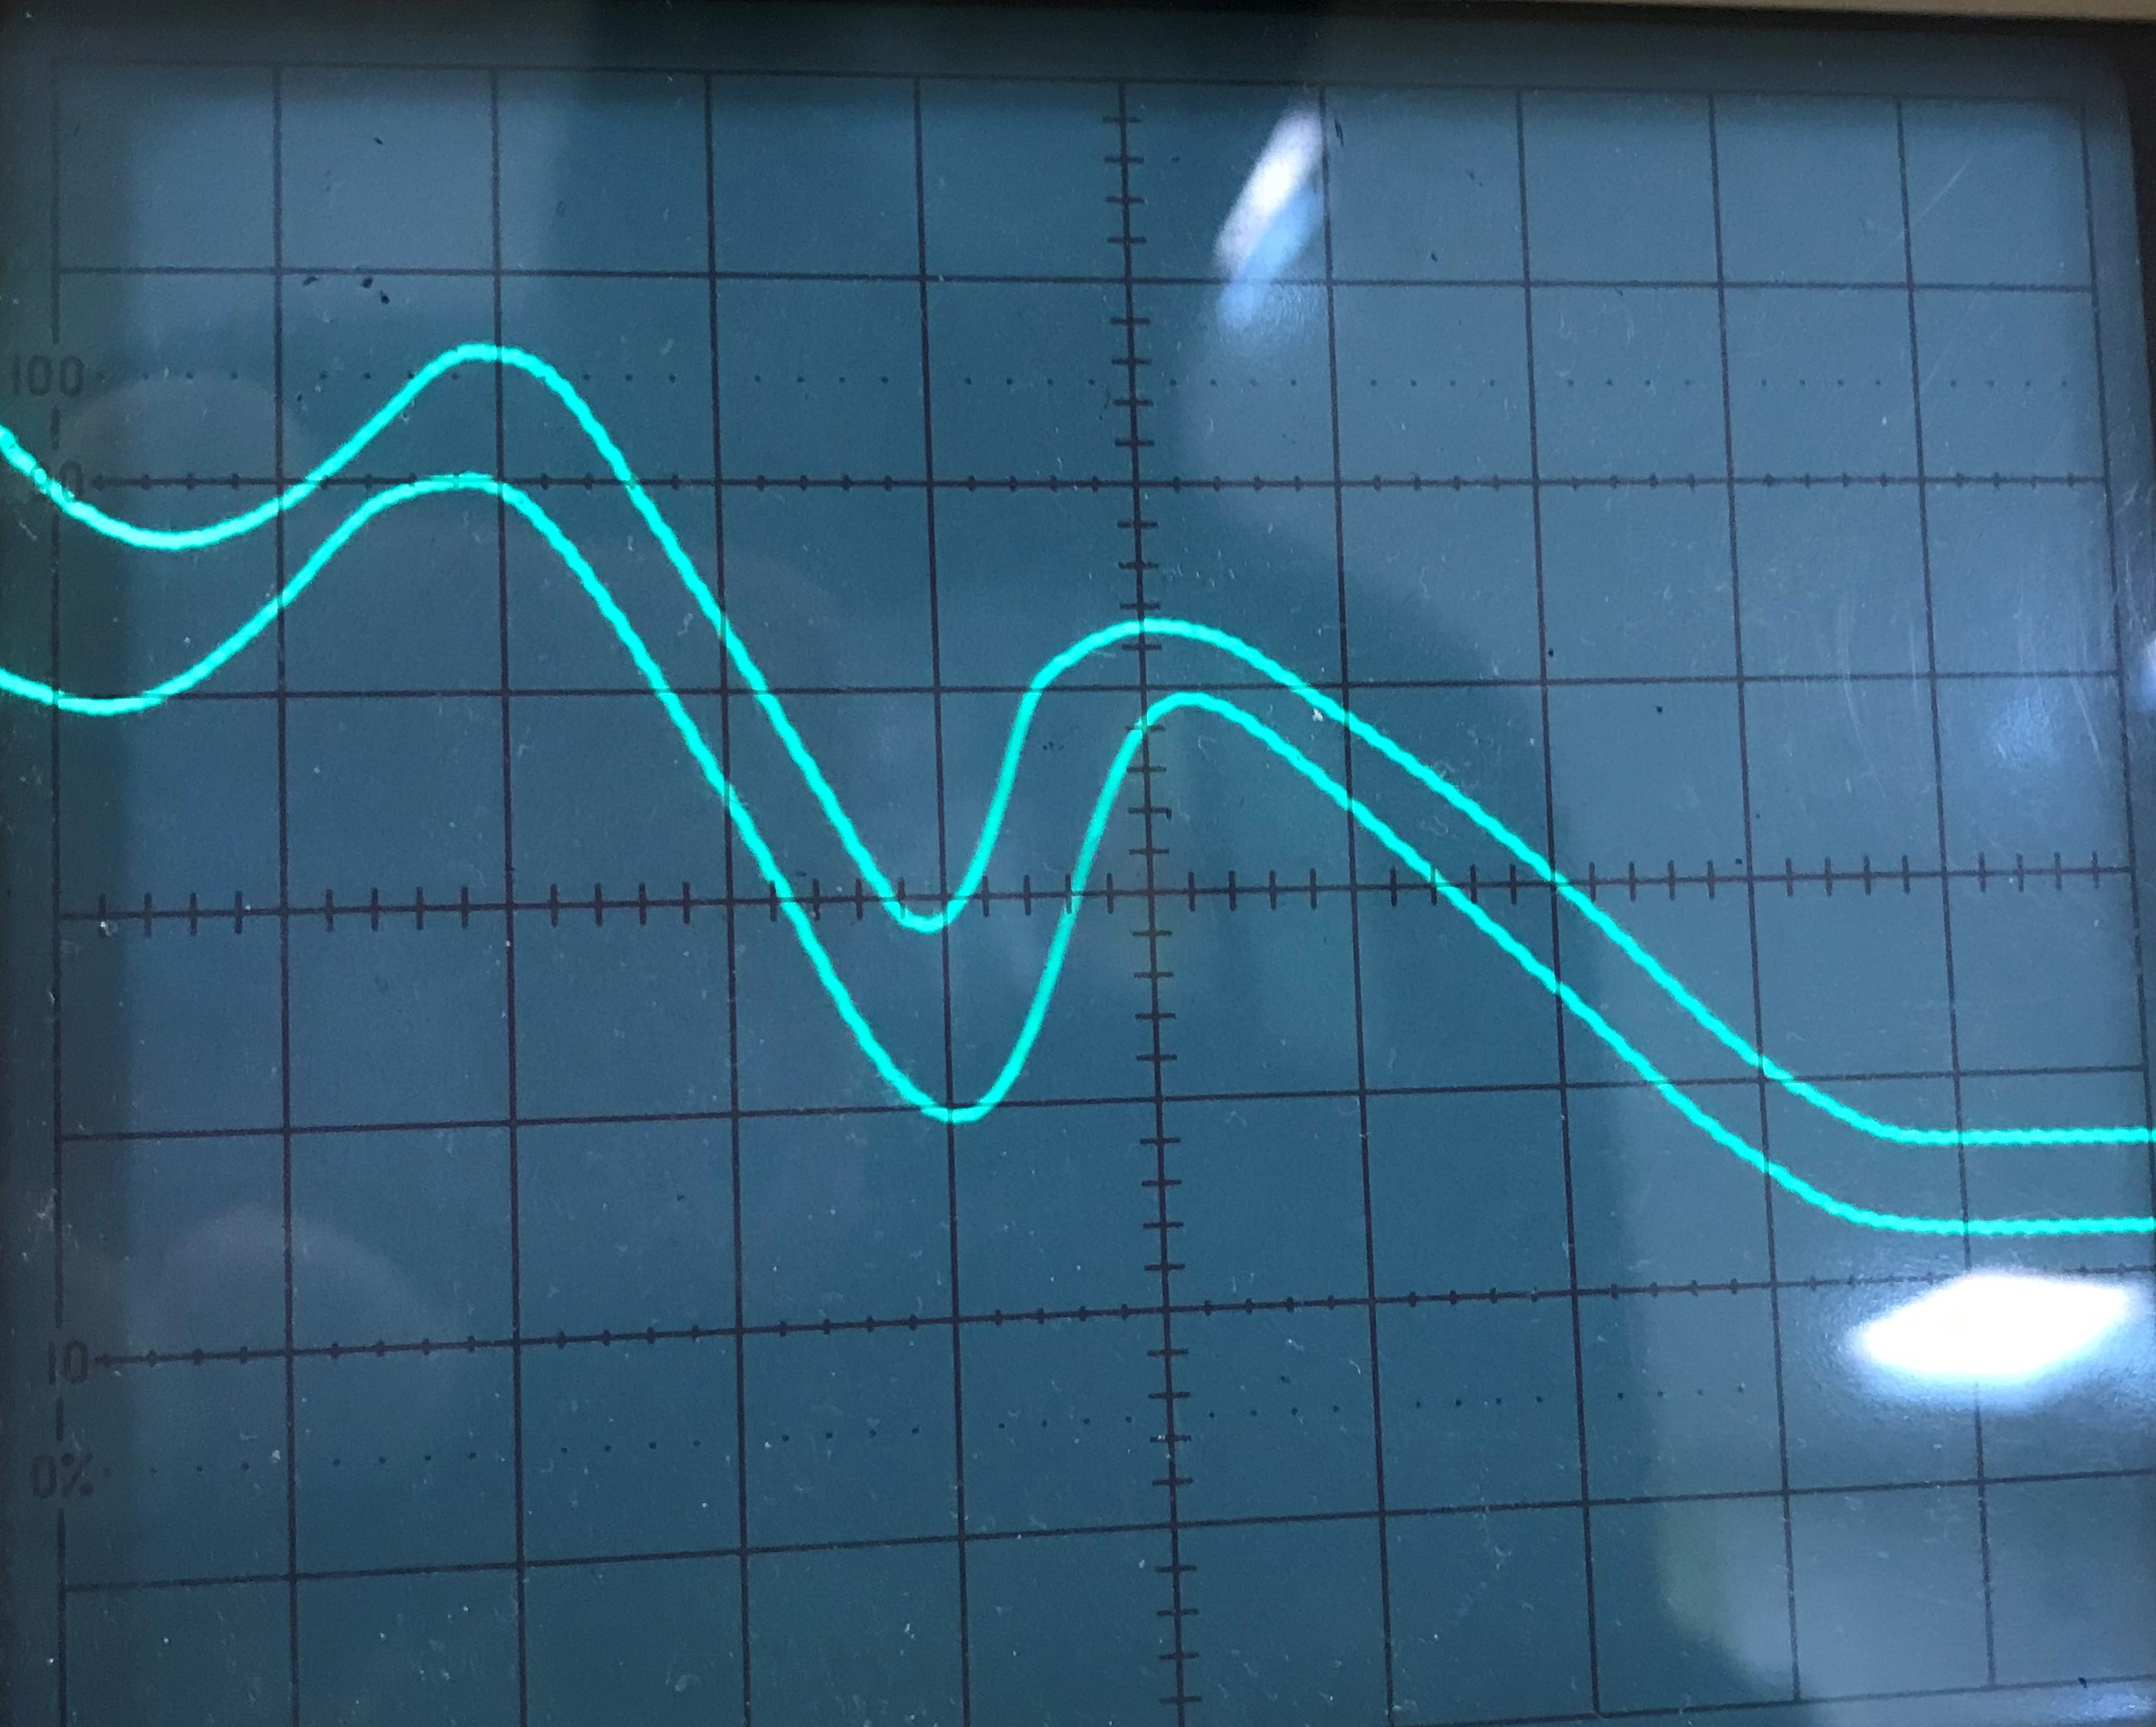
\includegraphics[width=\textwidth]{6}
                \caption{$U = 6V$}
            \end{minipage}
                \hfill
            \begin{minipage}{0.33\textwidth}
                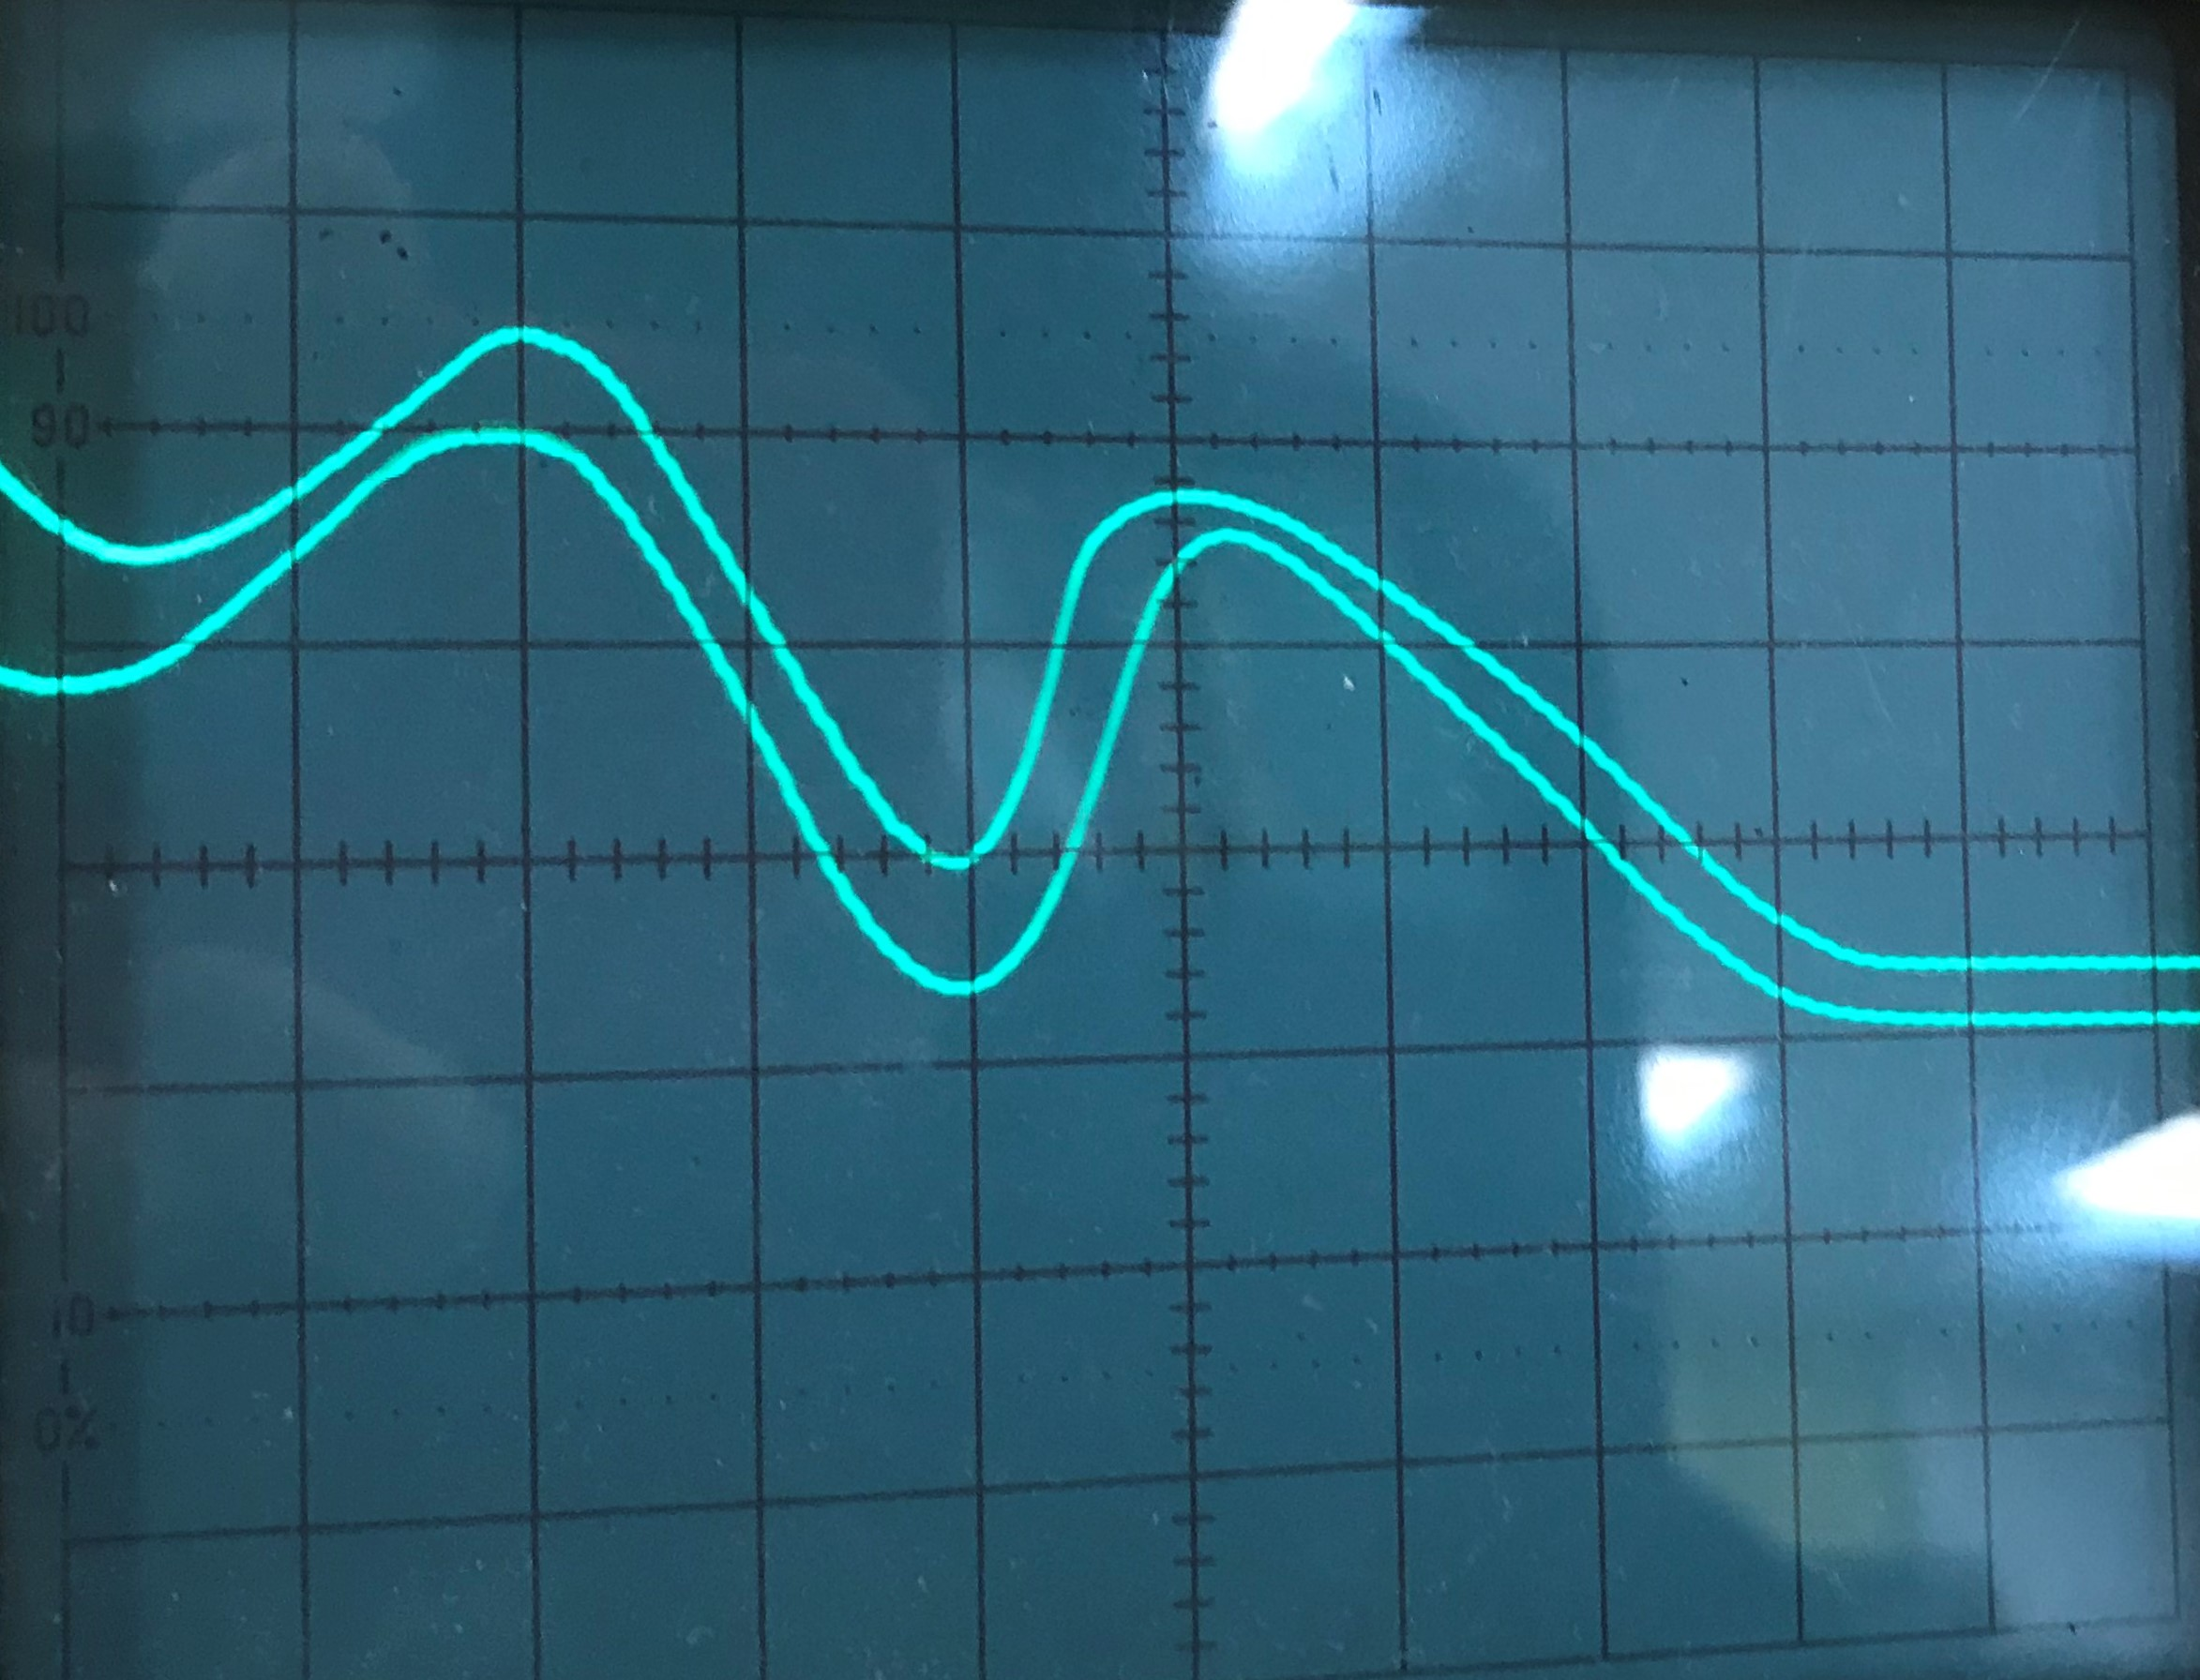
\includegraphics[width=\textwidth]{8}
                \caption{$U = 8V$}
            \end{minipage}
        \end{center}
    \end{figure}
    
    При максимальном ускоряющем напряжении измерим на экране расстояния
    между максимумами и между минимумами осциллограммы ($\Delta V$ в вольтах
    при установке ручкиплавной регулировки на максимум - до щелчка).

    \begin{table}[h!]
        \centering
        \caption{Измерение расстояний между максимумами и между минимумами}
        \label{my-label}
        \begin{tabular}{|c|c|c|c|c|c|c|}
            \hline
           $V_2$, \,\text{В} & $\Delta V_{max}$, \,\text{В} & $\Delta V_{min}$, \,\text{В} \\ \hline
            4    & $17.1 \pm 1.3$           & $19.8 \pm 1.3$           \\ \hline
            6    & $17.6 \pm 1.3$           & $20.5 \pm 1.3$            \\ \hline
            8    & $18.1 \pm 1.3$           & $22.5 \pm 1.3$           \\ \hline
        \end{tabular}
    \end{table}

    Отсюда получаем, что энергия возбуждения первого уровня атома гелия равна:
    \begin{equation*}
        E_1=20,93\pm 3,05 \,\text{эВ}         
    \end{equation*}
    Получим вольт-амперную характеристику $I_K=f(V_a)$ в статическом режиме.

    \begin{table}[h!]
        \caption{Измерения}
        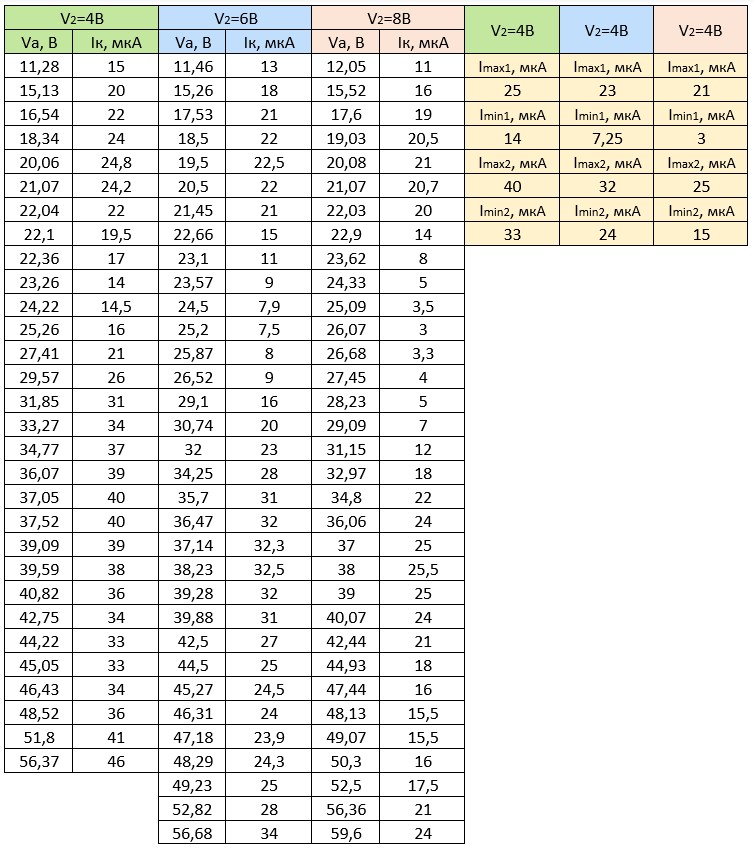
\includegraphics[width=\linewidth]{2020-11-01}
    \end{table}
    \pagebreak
    Построим по измеренным точкам графики.
    
    \begin{figure}[h!]
        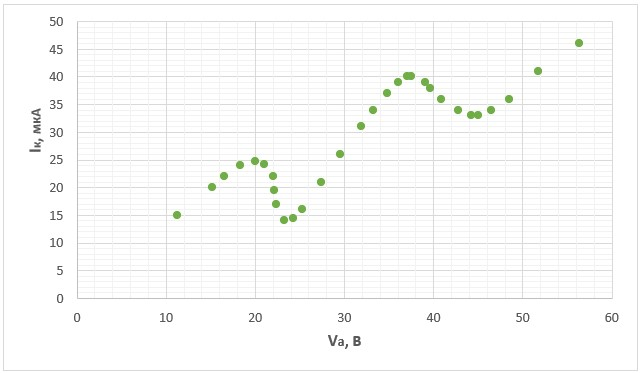
\includegraphics[width=\linewidth]{4V}
        \caption{$V_2 = 4B$}
    \end{figure}
    \pagebreak
    \begin{figure}[h!]
        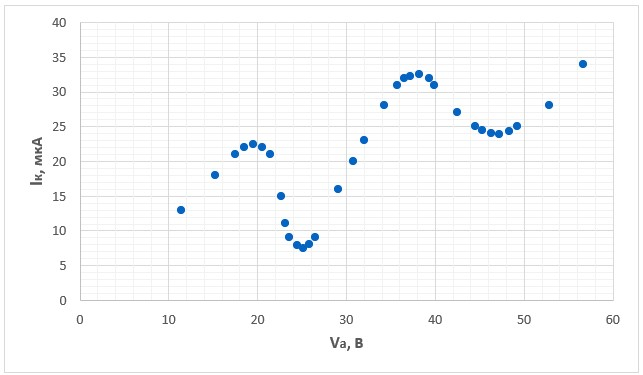
\includegraphics[width=\linewidth]{6V}
        \caption{$V_2 = 6B$}
    \end{figure}
    \pagebreak
    \begin{figure}[h!]
        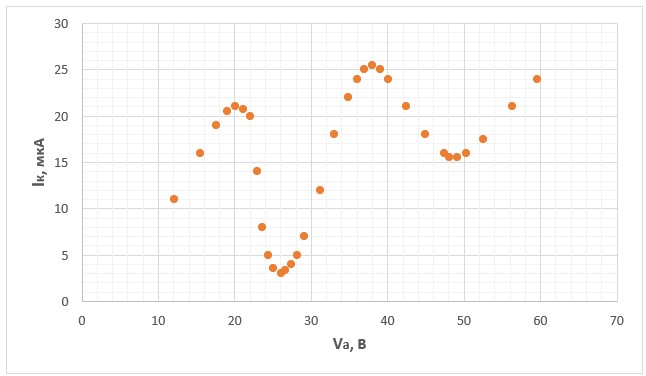
\includegraphics[width=\linewidth]{8V}
        \caption{$V_2 = 8B$}
    \end{figure}
    
    \begin{figure}[h!]
        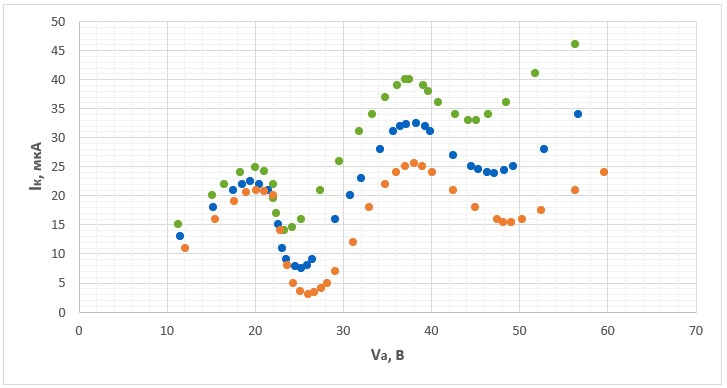
\includegraphics[width=\linewidth]{2020-11-01-2}
        \caption{$V_2 = 8B$}
    \end{figure}
    \pagebreak
    Определим по графикам энергию возбуждения первого уровня атома гелия.

    \begin{table}[h!]
        \centering
        \label{my-label}
        \begin{tabular}{|c|c|c|}
            \hline
           $V_2$, \,\text{В} & $\Delta V_{max}$, \,\text{В} & $\Delta V_{min}$, \,\text{В} \\ \hline
            4    & $16.8 \pm 0.8$           & $21.0 \pm 0.8$           \\ \hline
            6    & $18.3 \pm 0.8$           & $22.0 \pm 0.8$            \\ \hline
            8    & $17.5 \pm 0.8$           & $22.5 \pm 0.8$           \\ \hline
        \end{tabular}
    \end{table}

    Отсюда получаем, что энергия возбуждения первого уровня атома гелия равна:
    \begin{equation*}
    E_1=21,83\pm 0,84 \,\text{эВ}  
    \end{equation*}
\section{Вывод}
    При выполнении работы определили, что измерять возбуждения первого уровня атома
    водорода лучже по разности между минимумами, т.к. минимум на графике это как раз когда электроны теряют больше всего энергии (минимумы на графике как раз показывают момент когда у нас атомы переходят в возбужденное состояниец).
    Проделанная работа позволяет убедится в дискретности энергетических уровней в атоме гелия.
    Снятие вольт-амперной характеристики в динамическом режиме позволяет наглядно увидеть структуру энергетических уровней.
    Статический режим же нужен для более точного измерения энергии возбуждения атома.
    Эксперимент показал, что измеренная нами энергия атома близка к табличной
    (сходится по порядку величины).
			
\end{document}
